\textbf{Solution.}
\begin{enumerate}
  \item \textbf{ICE curves for $x_1$.} Plugging each category:
  \begin{align*}
    \hat f^{(a)}(x_1) &= 3 - 8x_1, & \hat f^{(b)}(x_1) &= 3 - 8x_1 + 16x_1 = 3 + 8x_1.
  \end{align*}
  They intersect at $x_1=0$ with value $3$. Slopes $-8$ vs $+8$ show a \emph{pure interaction}: the direction of effect of $x_1$ flips with $x_2$; no additive shift (same intercept 3).

  \item \textbf{Partial dependence of $x_1$.} Average over $X_2$:
  \begin{align*}
    \mathrm{PD}_{x_1}(t) &= 0.5(3 - 8t) + 0.5(3 + 8t) = 3.
  \end{align*}
  PDP is flat at 3 because opposite slopes cancel. This hides the strong conditional effects visible in ICE; inspecting ICE variance (here large) is critical to avoid concluding ``no effect''.
  \begin{figure}[h!]
    \centering
    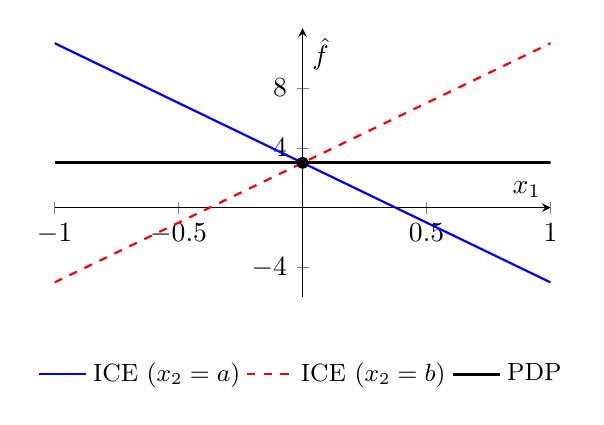
\begin{tikzpicture}
      \begin{axis}[
        width=0.65\textwidth,
        height=5.0cm,
        xmin=-1, xmax=1,
        ymin=-6, ymax=12,
        axis lines=middle,
        xlabel={$x_1$}, ylabel={$\hat f$},
        xtick={-1,-0.5,0,0.5,1},
        ytick={-8,-4,0,4,8},
        samples=101,
        domain=-1:1,
        legend style={draw=none,at={(0.5,-0.2)},anchor=north,legend columns=3,font=\small}
      ]
        \addplot[blue, thick] {-8*x + 3}; \addlegendentry{ICE ($x_2=a$)}
        \addplot[red, thick, dashed] {8*x + 3}; \addlegendentry{ICE ($x_2=b$)}
        \addplot[black, very thick] {3}; \addlegendentry{PDP}
        \addplot[only marks, mark=*, mark size=2pt] coordinates {(0,3)};
      \end{axis}
    \end{tikzpicture}
  \end{figure}
\end{enumerate}

